\documentclass{article}
\usepackage[dvipsnames]{xcolor}
\usepackage[paperwidth=20cm, paperheight=6.5cm, margin = 0cm, top=0.5cm]{geometry}

\usepackage{pgf}
\usepackage{tikz}
\usetikzlibrary{arrows,automata}
\usetikzlibrary{positioning}

\tikzstyle{source}  = [draw,circle,fill=black,thick,inner sep=0mm,minimum size=2mm]
\tikzstyle{box}  = [draw,rectangle,thick,inner sep=2mm,minimum width=8mm, minimum height=8mm]

\begin{document}
\begin{center}
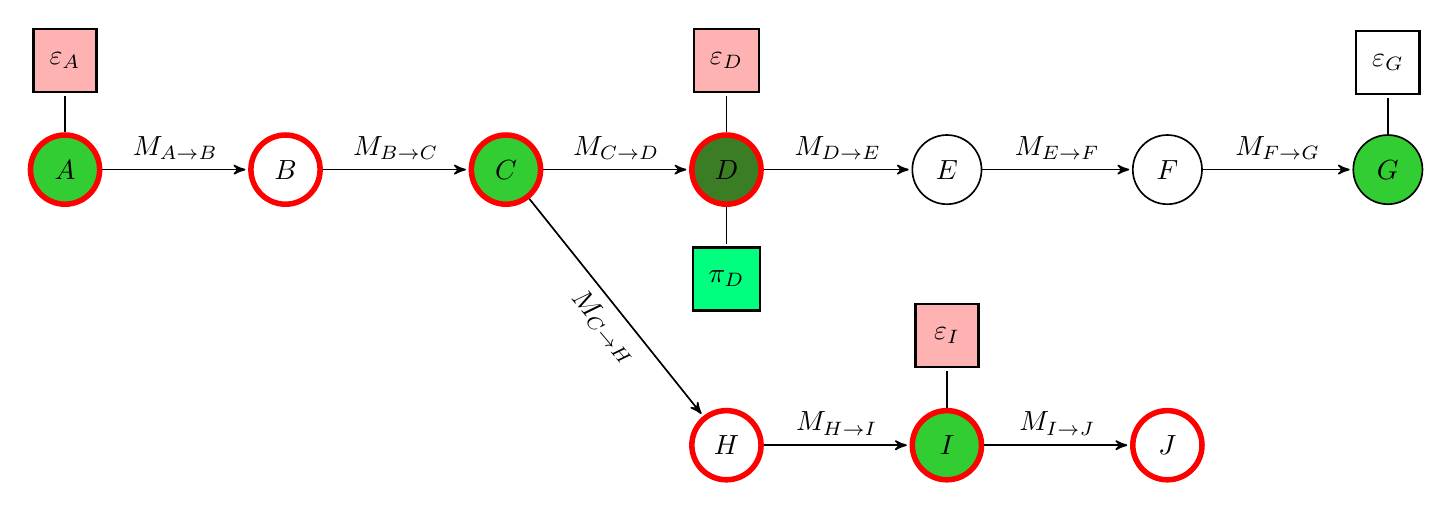
\begin{tikzpicture}[->,>=stealth',shorten >=1pt,auto,node distance=2.8cm,semithick]
                    
\node[state, fill=LimeGreen, draw=red, line width=2pt] (X1)               {$A$}; 
\node[state, draw=red, line width=2pt] (X2) [right of=X1] {$B$};                   
\node[state, fill=LimeGreen, draw=red, line width=2pt] (X3) [right of=X2] {$C$};                   
\node[state, fill=OliveGreen, draw=red, line width=2pt] (X4) [right of=X3] {$D$};                   
\node[state] (X5) [right of=X4,] {$E$}; 
\node[state] (X6) [right of=X5,] {$F$}; 
\node[state, fill=LimeGreen] (X7) [right of=X6,] {$G$}; 

\node[state, draw=red, line width=2pt] (Y4) [below=3.5cm of X3, right of=X3] {$H$};                   
\node[state, fill=LimeGreen,  draw=red, line width=2pt] (Y5) [right of=Y4] {$I$};                   
\node[state, draw=red, line width=2pt] (Y6) [right of=Y5] {$J$};

\node[box, fill=red, opacity=0.3, text opacity=1, draw opacity=1][above=0.5cm of X1](E1){$\varepsilon_A$};                  
\node[box, fill=red, opacity=0.3, text opacity=1, draw opacity=1][above=0.5cm of X4](E4){$\varepsilon_D$};                  
\node[box][above=0.5cm of X7](E7){$\varepsilon_G$};                  
\node[box, fill=red, opacity=0.3, text opacity=1, draw opacity=1][above=0.5cm of Y5](D5){$\varepsilon_I$};                  


\node[box, fill=SpringGreen][below=0.5cm of X4](P4){$\pi_D$};                  


\path
	(X1) edge node {$M_{A\to B}$} (X2)
	(X2) edge node {$M_{B\to C}$} (X3)
	(X3) edge node {$M_{C\to D}$} (X4)
	(X4) edge node {$M_{D\to E}$} (X5)
	(X5) edge node {$M_{E\to F}$} (X6)
	(X6) edge node {$M_{F\to G}$} (X7);

\path
	(X3) edge node[yshift=+0.1cm, xshift=-0.8cm, rotate=-50] {$M_{C\to H}$} (Y4)
	(Y4) edge node {$M_{H\to I}$} (Y5)
	(Y5) edge node {$M_{I\to J}$} (Y6);


\path
	(X1) edge[-] (E1)
	(X4) edge[-] (E4)
	(X7) edge[-] (E7);

\path
	(Y5) edge[-] (D5);

\path
	(X4) edge[-] (P4);


\end{tikzpicture}
\end{center}

\end{document}
